\subsection{User Interface Toolbox}\label{sec:UI}
The key goal of the UI module is to offer a user friendly, efficient and uniform point of access to the DA, which can be optimized for the current manufacturing environment, task and operator. Therefor, we provide a toolbox for adaptable multimodal UIs that can be rendered on multiple devices and support seamless two-way interaction.

The focal element in the architectural framework behind our UI toolbox (see Figure~\ref{fig:ui-architecture}) is the back-end C\# WPF application that serves as an encapsulating entity for a SignalR hub. It functions as the central authority and communication hub, governing all communication processes initiated by individual clients. There are no limitations for the type of devices that can act as a client, apart from being able to communicate through SignalR~\cite{SignalR01,Sharma_2023}. We implemented a toolbox of reusable components on the Microsoft MAUI platform~\cite{Maui01,Maui02}, with support for an extensive set of devices (e.g., desktop systems, tablets, smartphones, smartwatches), each with their own modalities, capabilities and strengths. The modular basis of the toolbox allows easy integration of other platforms and devices, including devices with limited modalities (e.g., a microcontroller directing an industrial signal tower).

While all clients are inherently equivalent, some can be defined to support more actions than others. One such client in our framework acts as a \emph{Wizard of Oz} and allows a supervising user to change the state, context and content of the system. The primary use case for this Wizard is to be able to conduct user tests with features, that might not yet have been fully implemented, but that are emulated or manipulated by the Wizard (thus facilitating rapid prototyping).
Another example of such a client is one that acts as a \emph{Bridge to the Operator Service Bus}. Communication to the other components of the project can be done through any communication channel (e.g. MQTT, REST, ...) and the bridge handles any translations from the external data to their internal representations (if deemed useful) before triggering actions within the system.

\begin{figure}
    \centering
    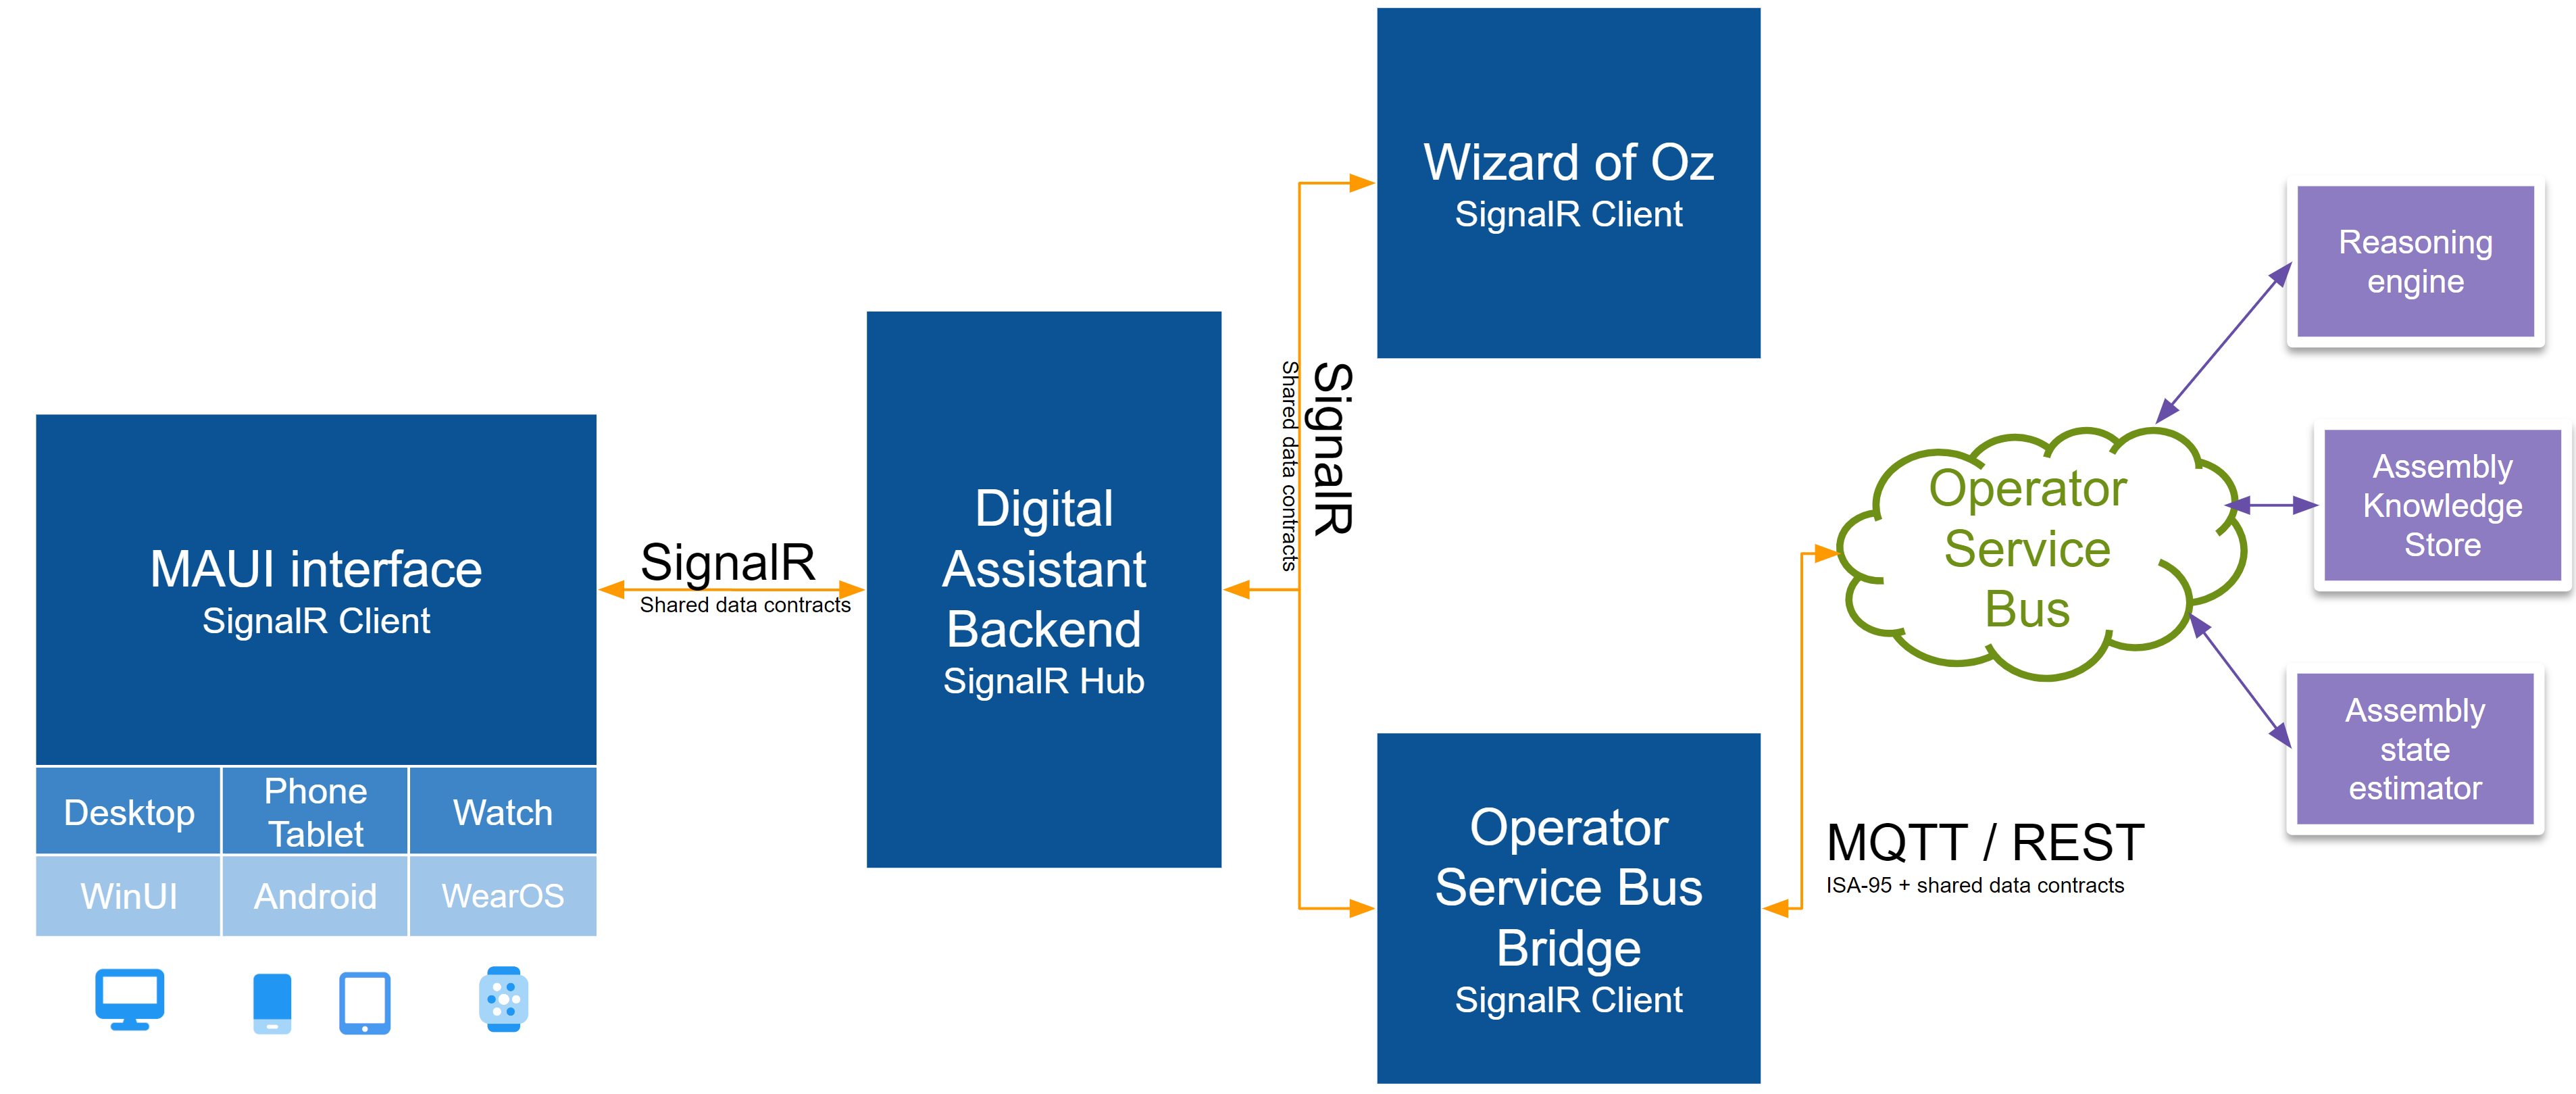
\includegraphics[width=1\linewidth]{figs/UI-architecture.png}
    \caption{Architectural framework behind our UI toolbox.}
    \label{fig:ui-architecture}
\end{figure}

Due to the heterogeneity of working environments, assembly tasks and operators, we focus on a toolbox that supports adaptable UIs to ensure a consistent and usable experience in a large variety of circumstances, as discussed in Section~\ref{sec:DA}. As the context of use is a fluid concept, our toolbox aims for a maximum degree of flexibility. For instance, the operator or manufacturing company can decide on which devices will be used, depending on the given context of use and availability of devices. Regarding modalities, we aim for redundancy and flexibility for an operator to interact with the DA, as some modalities might be impaired by contextual limitations (e.g., when voice input fails because of too much ambient noise, a gesture can be used instead).

Our toolbox allows for an extensive configuration of devices and modalities (e.g., which modalities should be enabled and which output should be rendered on a particular device). Furthermore, should a device or modality suddenly become unavailable, the toolbox facilitates graceful degradation and quick reconfiguration. We implemented this flexibility by creating an \emph{Interaction Event Orchestrator (IEO)} that takes the known contextual parameters into consideration to determine the best device to respond to a given input interaction. The IEO requires a device to register its modalities and capabilities, ensuring it has the necessary information available.

We use the data provided by the clients to map all the possible interactions (and their corresponding modalities) at a certain moment in time and provide it to the operator. The available interactions will vary, depending on the state and content of the application (e.g., a thumbs up gesture will signal a positive feedback to provided assistance, but might not have any effect when the operator is reading a manual). 
Additionally, after an interaction is handled, the IEO also provides information about what just happened (and by which device) so the operator can learn about the system and diagnose any unexpected results. In future work, this information could then be used to adapt and fine-tune the system's response for future events.

In addition to the reactive nature of the system, the platform also supports providing proactive assistance, which entails different notification types and urgency levels. 
The operator could, for example, receive an informative message that appears in a queue to be read at a time of the operator's discretion; the system will not try to get the attention of the operator in such an event. 
Alternatively a critical warning might need to be delivered to the operator because a potentially dangerous action was detected. In the latter case, an appropriate set of the available devices and modalities should be used to get the attention of the operator as soon as possible.
Another category of notifications are those that are quite important but not very urgent, and are therefore not warranted to interrupt the operator in his current task. This information should rather be communicated to the operator at a more \textit{opportune time}, which can be approximated by processing information on the user’s current environment \cite{lindlbauer2019ContextAwareOnlineAdaptation}, the state estimation of the task and proxemics \cite{Marquardt_2015} \cite{Williamson_2022}. 
To avoid cognitive overload, it might be a good idea to group the available notifications so the interruption, that could not be prevented, is at least used optimally.
Furthermore the perceived progress of the state estimation might give a good lead to find a natural breakpoint in the execution of the task at hand.
From the state estimator we also have access to the coordinates of the operator and the devices in the environment, which enables us to determine which devices are still within the active range (i.e., in view and/or in interaction range) of the operator and, in contrast, which can be considered as a dormant device. These dormant devices can then be handled differently (or even ignored) when trying to find the best device to signal a notification to the operator.

\iffalse
\textit{A major benefit of the DA is the on-demand, reactive nature of support, as nonstop support can negatively influence task completion time and perceived cognitive load [32]. The downside is that info might be overlooked by the operator. Therefore, the DA will offer proactive assistance when needed (e.g., in case of errors in task execution) [33], [34]. We will investigate decision strategies that use implicit inputs such as cognitive load [35], state estimation and proxemics\textcolor{red}{refs}. 
Proactivity, however, will always be imperfect, akin to inevitable flaws in activity and context detection: we will implement a two-way feedback loop, so the operator can complement or correct info (e.g., in case of low confidence level of an activity recognition or additional information offered because of a lack of experience, the operator is made aware and can intervene). }

\textit{We will also implement strategies to attune the output to the context of use (e.g., the operator's experience, the task's criticality, the probability of errors). To this end, we will render information with various levels of detail [37], [38], adapted to a manufacturing setting and augmented with a mixed-initiative approach to keep the operator in control. An inexperienced operator, for instance, will be offered more detailed information (e.g., instructional video or diagram instead of text) and more frequent proactive suggestions, but the operator can always intervene to avoid unwanted or unneeded behavior.}


Leveraging multiple modalities and devices in combination with a conversational UI allows seamless interaction [26], as well as taking advantage of fitting technologies in different situations [27]. Therefore, we will support multiple devices and modalities to interact with the DA, using web-based multi-device formats. Interaction between the operator and DA will always happen through a UI on a device, which needs to be created for and tailored to that specific device for an optimal experience. Automatic UI creation and adaptation mechanisms, however, are error prone and complex, and lack control, transparency and predictability [28]. On the work floor, operators require stable interfaces that are predictable. Therefore, we focus on an adaptable
UI [29] and design templates that take into account best practices [30]to ensure a consistent and usable experience. 
In contrast to existing work, we will use a holistic approach that considers (i) context, devices, modalities, and UI together, (ii) from both a technical and usability perspective, (iii) in a manufacturing setting: we will provide a toolbox for multimodal UIs that can be rendered on multiple devices and support seamless two-way interaction, which can be ‘optimized’ for the current manufacturing environment, task and operator (see figure 1 for a practical example).



A major benefit of the DA is the on-demand, reactive nature of support, as nonstop support can negatively influence task completion time and perceived cognitive load [32]. The downside is that info might be overlooked by the operator. Therefore, the DA will offer proactive assistance when needed (e.g., in case of errors in task execution) [33], [34]. We will investigate decision strategies that use implicit inputs such as cognitive load [35] and state estimation. Proactivity, however, will always be imperfect, akin to inevitable flaws in activity and context detection: we will implement a two-way feedback loop, so the operator can complement or correct info (e.g., in case of low
confidence level of an activity recognition or additional information offered because of a lack of experience, the operator is made aware and can intervene). 

To process both explicit and implicit inputs, we will build on our experiences with prototyping multimodal interactions [36], as it is not our goal to advance the state of the art with regard to low-level input processing. We will also implement strategies to attune the output to the context of use (e.g., the operator's experience, the task's criticality, the probability of errors). To this end, we will render information with various levels of detail [37], [38], adapted to a manufacturing setting and augmented with a mixed-initiative approach to keep the operator in control. An inexperienced operator, for instance, will be offered more detailed information (e.g., instructional video or diagram instead of text) and more frequent proactive suggestions, but the operator can always intervene to avoid unwanted or unneeded behavior.



Topics to handle:
\begin{itemize}
    \item Multi device
    \begin{itemize}
        \item Flexibility (use it or don't)
    \end{itemize}
    \begin{itemize}
        \item Graceful degradation (a device was removed from the scene)
    \end{itemize}
    \item multimodal
    \begin{itemize}
        \item redundancy (e.g. if voice doesn't work, use a gesture/...)
        \item provide insight into what's possible at a certain time (with which modalities)
        \item provide information about what just happened
    \end{itemize}
    \item give insight into current assembly state
    \begin{itemize}
        \item 2 way feedback loop
    \end{itemize}
    \begin{itemize}
        \item proxemics to take position of the operator into account?
    \end{itemize}
    \item Reactive <> proactive
    \begin{itemize}
        \item Proactivity:
        \begin{itemize}
            \item interruptability - opportune time to interrupt the user
        \end{itemize}
    \end{itemize}
\end{itemize}
\fi